\section{Laboratory Lecture 4: Stepper Motor Controller}

The main objective of this practice is to understand the fundamentals of Finite State Machines and their main applications. We will then use the knowledge that we have acquired to build a stepper motor controller which will be controlled by a rotary encoder.

\subsection{Finite State Machines}

Before diving into the practice, we must firstly define what a Finite State Machine. In essence, a FSM is a machine that makes predictable transitions through a sequence of states, based on external inputs and the current state of the machine. In digital electronics, the timing of the transition of the machine from one state to another is controlled by a register and a system clock, while the next state of the machine is determined by a combination of logic gates and embedded memory. The number of states, as the name suggests can be assumed to be finite. ~\autocite{FSM} \medskip

Two basic types of state machines are the Moore and the Mealy. The Moore state machine is one where the outputs depend only on the internal present state. The Mealy state machine is one where the outputs depend on both the internal present state and on the inputs. ~\autocite{FLOYD} \medskip

We can see and example of these type of machines here:


\begin{figure}[H]
    \centering
    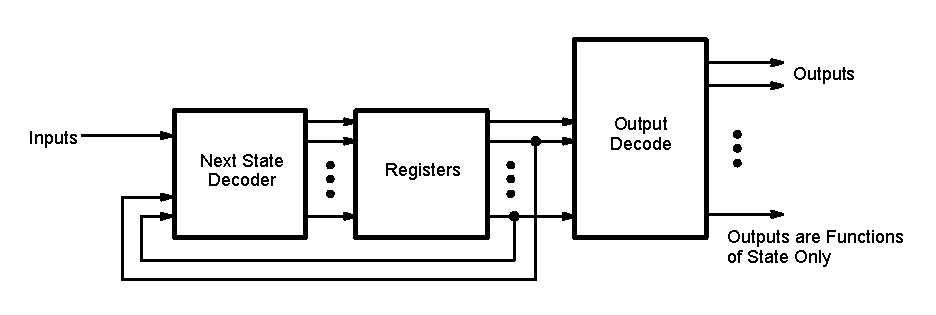
\includegraphics[width = \textwidth]{Graphics/Practice 4/MOORE.pdf}
    \caption{Moore State Machine Operation Diagram ~\autocite{AMD}}
    \label{fig:MOORE}
\end{figure}

\vspace{-0.3cm}

\begin{figure}[H]
    \centering
    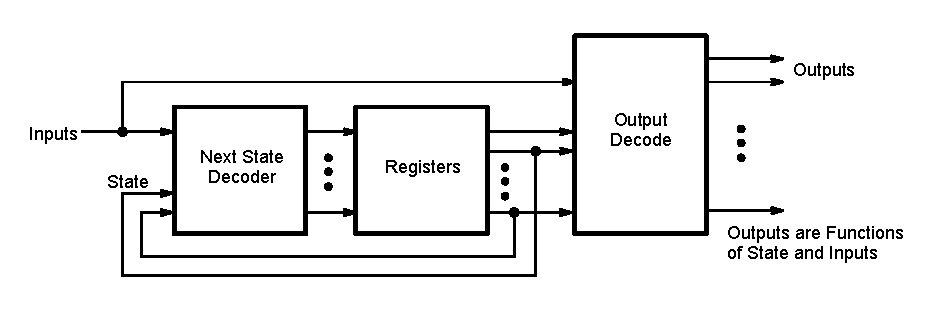
\includegraphics[width = \textwidth]{Graphics/Practice 4/MEALY.pdf}
    \caption{Mealy State Machine Operation Diagram ~\autocite{AMD}}
    \label{fig:MEALY}
\end{figure}


To represent both types of machines, a State Diagram is used. Normally, state diagrams are composed of bubbles, which indicate the different states, and arrows, that indicate the transitions.\medskip

In the following example we will implement a FSM that recognizes the sequence "10" using both type of machines.

\begin{figure}[H]
    \centering
    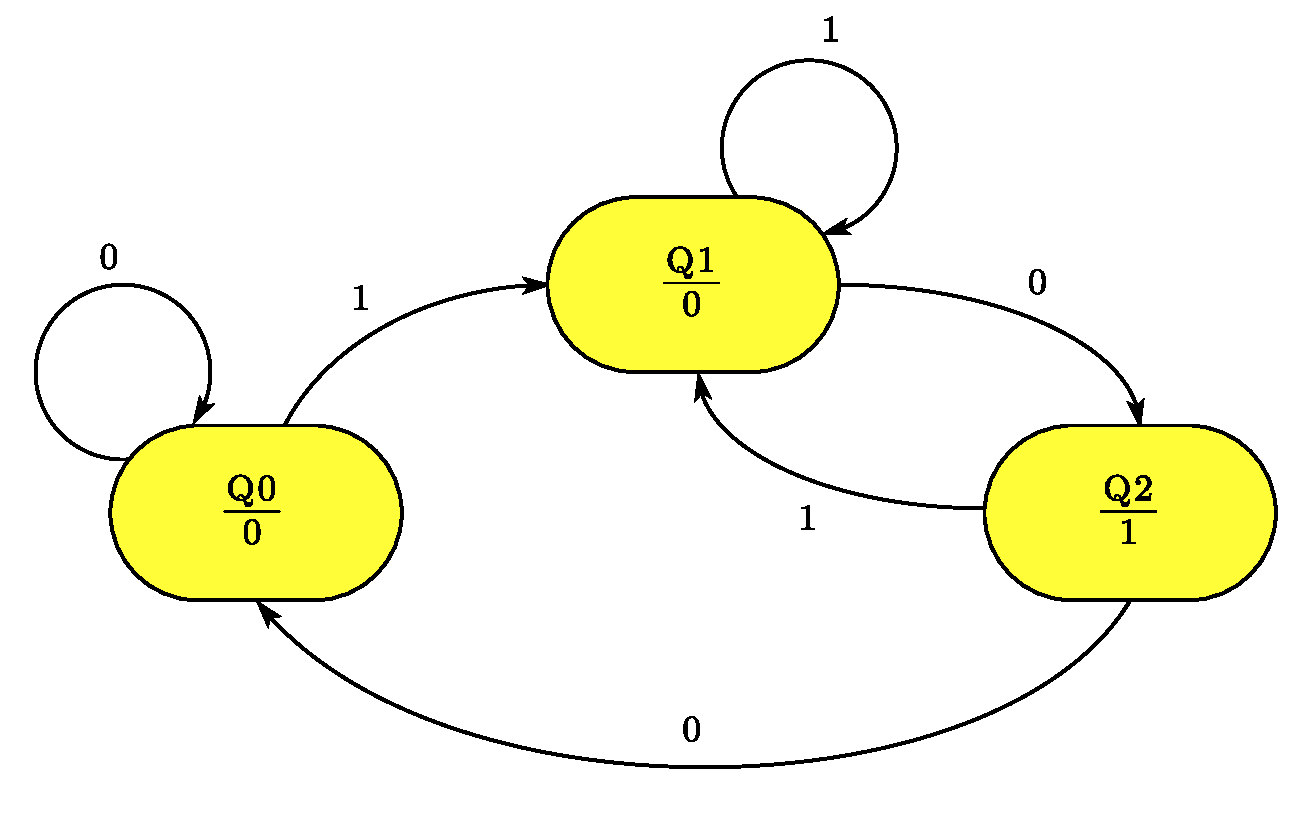
\includegraphics[scale = 0.55]{Graphics/Practice 4/MOORE_FSM.pdf}
    \caption{Moore State Machine ~\autocite{SLIDES_4}}
    \label{fig:MOORE}
\end{figure}

For this particular case, \bm{$Q_0$} means \textit{No elements in the sequence observed}, \bm{$Q_1$} means \textit{"1" observed} and \bm{$Q_2$} means \textit{"10" observed}

\vspace{-0.3cm}

\begin{figure}[H]
    \centering
    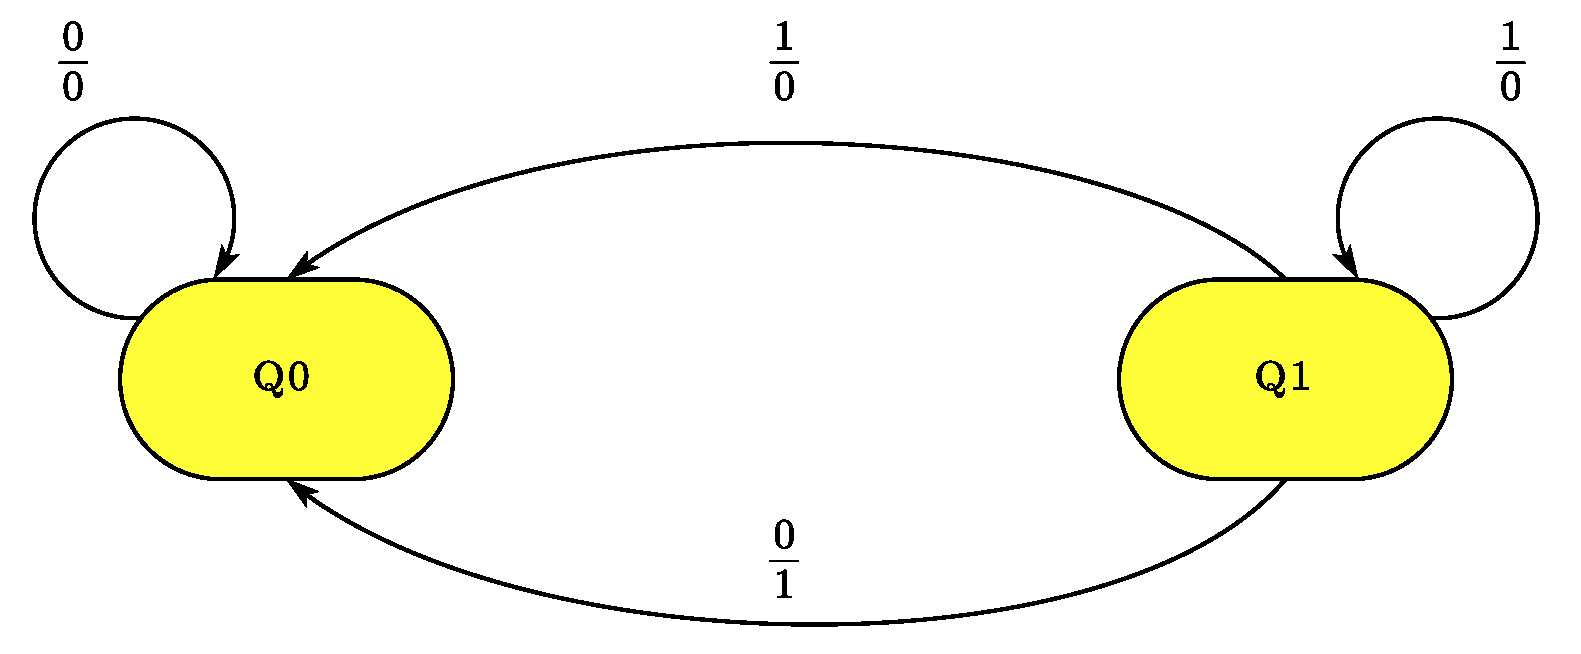
\includegraphics[scale = 0.45]{Graphics/Practice 4/MEALY_FSM.pdf}
    \caption{Mealy State Machine ~\autocite{SLIDES_4}}
    \label{fig:MEALY}
\end{figure}

In the latter case, the states mean the same, but as we can seem there is one less state than in the previous one. \medskip

\clearpage

This brings us to the advantages and disadvantages that both of them have:

\begin{enumerate}
    \item Mealy machines have \textbf{fewer states} and react faster to inputs.
        \begin{itemize}
            \item Outputs are defined in the transitions ($n^2$) rather than in the state itself ($n$).
            \item They react in the same cycle, i.e., they do not need to wait for the clock.
            \item Their outputs may be considerably shorter than the clock cycle, which can pose problems.
            \item Since fewer states than the \textbf{Moore} type are used, the propagation delay time is also shorter.
        \end{itemize}
    \item Moore machines are \textbf{safer} to use.
        \begin{itemize}
            \item Outputs change at clock edge.
            \item In \textbf{Mealy machines}, an input change will cause an output change as soon as the logic is done, which a big problem when two machines are interconnected since asynchronous feedback may occur if one is not careful.
        \end{itemize}
\end{enumerate}

\clearpage

\subsection{Incremental encoder}

An incremental encoder is a type of rotary encoder that indicates both the ocurrence and the direction of movement. An encoder of such type does not indicate the absolute position or angle; it only reports changes in position and for each position, the direction of movement. \medskip

They usually have 2 outputs, \textit{A} and \textit{B}, which value changes as the encoder is swept through its range, incrementing the count every time that its shaft changes position.\medskip

\vspace{-0.5cm}

\begin{figure}[H]
    \centering
    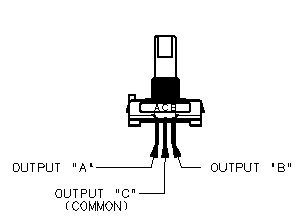
\includegraphics[scale = 1.3]{Graphics/Practice 4/ENCODER_DRAWING.pdf}
    \caption{Encoder pinout ~\autocite{ENCODER}}
    \label{fig:ENCODER_PINOUT}
\end{figure}

Incremental encoders output a defined number of pulses per revolution. We can use these pulses to obtain both the angle and the direction of the rotarion since the outputs \textit{A} and \textit{B} are shifted 90\textdegree. This behaviour can be clearly seen in the following graph:\medskip

\begin{figure}[H]
    \centering
    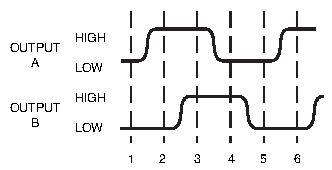
\includegraphics[scale = 1.5]{Graphics/Practice 4/ENCODER_POSITION.pdf}
    \caption{Encoder Output States ~\autocite{ENCODER}}
    \label{fig:ENCODER_STATES}
\end{figure}

\clearpage

\subsection{Exercise 1: Motor Control}

Now that we have defined how every part of the system works, we will move onto solving the laboratory lecture itself. \medskip

The first and only exercse states the following:\medskip

\textit{Design a state machine (FSM) that supplies the proper output to a stepper motor according to the position of the incremental encoder. Draw the FSM.} \medskip

\textbf{\large Answer to Exercise 1:}\medskip

As per usual, we will implement the code for the FSM in VHDL and we will program it into a GAL22V10C. \medskip

The VHDL code can be found below:\medskip

\inputcode{VHDL/ENCODER.vhd}

As we can clearly see in the code, this FSM is of the type Moore, as the outputs update in the states themselves rather than in the transitions. In addition, since the capacity of the GALs is very limited, we have not added an asynchronous nor synchronous reset pin, which could cause problems in other, more complex FSMs.  \medskip

The output signal \textbf{STEPPER} will be connected to the stepper motor driver that we saw in the last practice so as to simulate a similar version of the full-step control mode with fewer states (\textbf{See Subsubsection \ref{sec:FULL_STEP} for more on this})\medskip

The State Diagram that describes this FSM can be found below:

\begin{figure}[H]
    \centering
    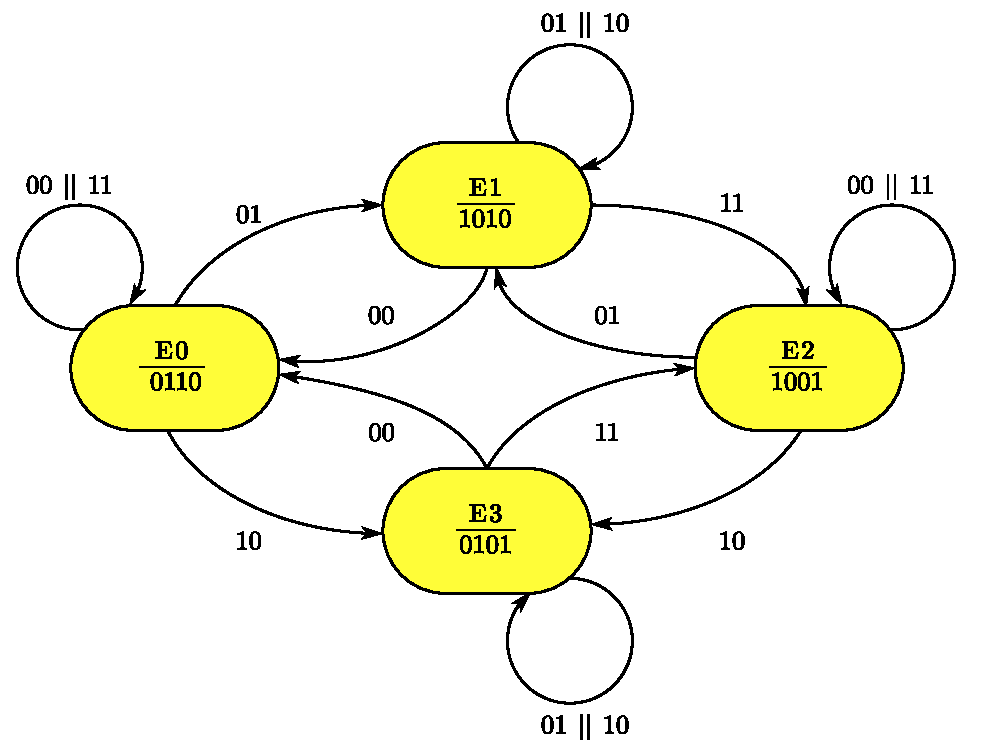
\includegraphics[scale = 0.75]{Graphics/Practice 4/EXERCISE_FSM.pdf}
    \caption{Stepper Controller with Incremental Encoder FSM}
    \label{fig:ENCODER_FSM}
\end{figure}

\clearpage